\vspace*{20pt}

\begin{figure}[!h]
\centering
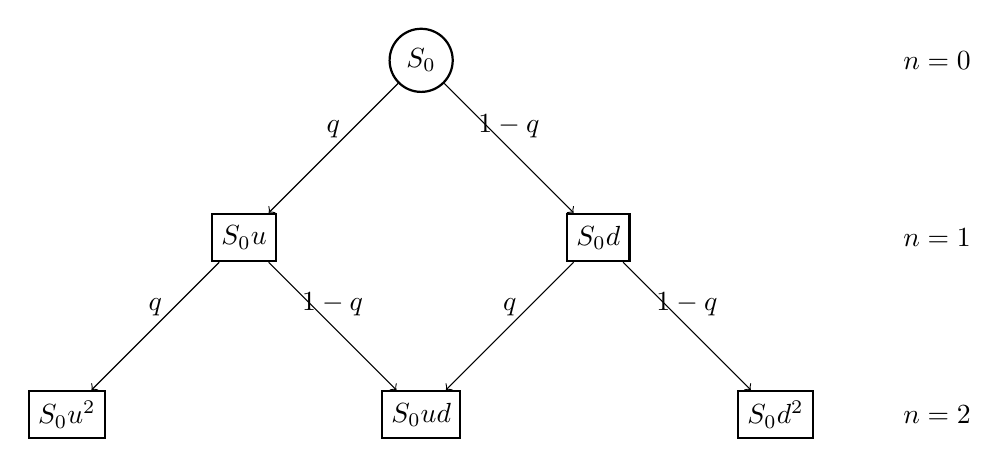
\begin{tikzpicture}[
    roundnode/.style={circle, draw=black, thick, minimum size=6mm},
    squarednode/.style={rectangle, draw=black, thick, minimum size=6mm},
    scale=1.5
  ]
  
  %Nodes
  \node[roundnode] at (0,0) (A) {$S_0$};
  \node[squarednode] at (-1.5,-1.5) (B) {$S_0 u$};
  \node[squarednode] at (1.5,-1.5) (C) {$S_0 d$};
  \node[squarednode] at (-3,-3) (D) {$S_0 u^2$};
  \node[squarednode] at (0,-3) (E) {$S_0 ud$};
  \node[squarednode] at (3,-3) (F) {$S_0 d^2$};
  
  %Lines
  \draw[->] (A) -- (B) node[midway,above] {$q$};
  \draw[->] (A) -- (C) node[midway,above] {$1-q$};
  \draw[->] (B) -- (D) node[midway,above] {$q$};
  \draw[->] (B) -- (E) node[midway,above] {$1-q$};
  \draw[->] (C) -- (E) node[midway,above] {$q$};
  \draw[->] (C) -- (F) node[midway,above] {$1-q$};
  
  %Labels
  \node[right] at (4,0) {$n=0$};
  \node[right] at (4,-1.5) {$n=1$};
  \node[right] at (4,-3) {$n=2$};

\end{tikzpicture}
\caption{Representation of the binomial tree with n=2} 
\label{fig:bin_tree}
\end{figure}

\vspace*{20pt}